\subsubsection{UC\theuccount-PG - GitLab segnala un evento di push a Producer GitLab}
%	\begin{figure}[H]
%		\centering
%		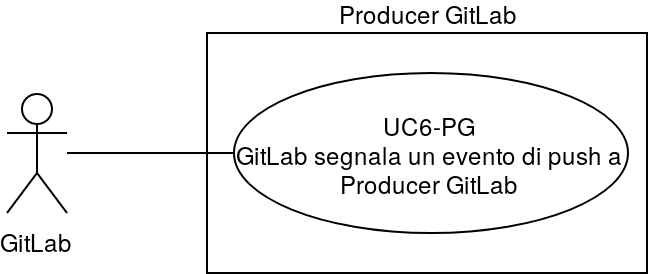
\includegraphics[width=0.5\textwidth]{img/casi_d'uso/UC6.png}\\
%		\caption{UC\theuccount-PG - GitLab segnala un evento di push a Producer GitLab}
%	\end{figure}
	\begin{itemize}
		\item \textbf{Codice}: UC\theuccount-PG.
		\item \textbf{Titolo}: GitLab segnala un evento di push a Producer GitLab.
		\item \textbf{Attori primari}: GitLab.
		\item \textbf{Descrizione}: GitLab segnala un evento di push tramite webhook a \progetto. L'evento di	push può essere composto da uno o più commit.
		I campi di interesse sono:
		\begin{itemize}
			\item Object kind
			\item Project
			\item Repository
			\item Commits
		\end{itemize}
		E in questo caso il campo object kind contiene ``push''.
		\item \textbf{Precondizione}: Viene effettuato un push su GitLab da segnalare a \progetto.
		\item \textbf{Postcondizione}: il Producer GitLab riceve la segnalazione da GitLab.
		\item \textbf{Scenario principale}: 
		\begin{enumerate}
			\item Viene effettuato un push in GitLab
			\item GitLab procede all'invio della segnalazione di push al Producer GitLab
		\end{enumerate}
		
	\end{itemize}